\begin{SCfigure}
 \centering
    \begin{subfigure}[b]{0.3\textwidth}
        \centering
    	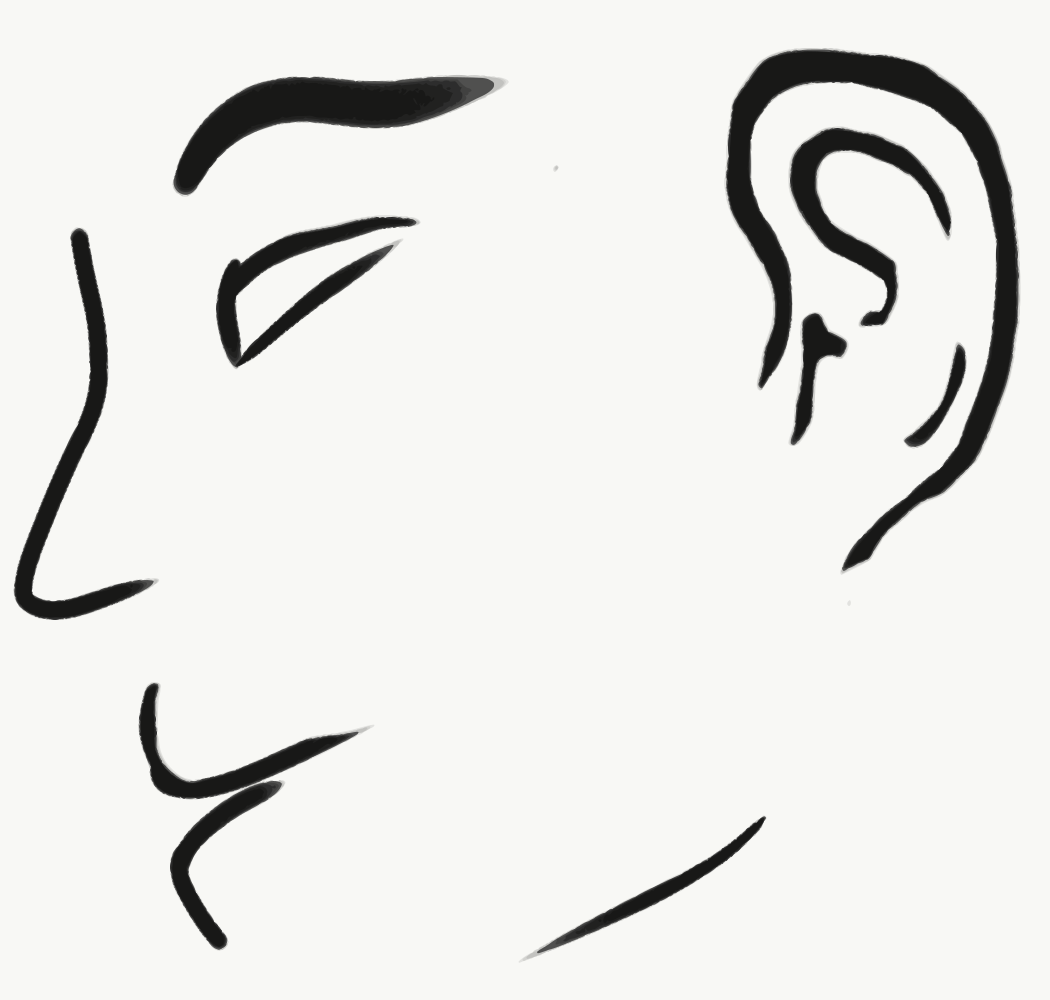
\includegraphics[width=\textwidth]{img/attached_earlobe}
        \caption{attached earlobe}
        \label{subfig:attached_earlobe}
    \end{subfigure}%
    \hspace{1em}
    \begin{subfigure}[b]{0.3\textwidth}
        \centering
        
\includegraphics[width=\textwidth]{img/detached_earlobe}
        \caption{detached earlobe}
        \label{subfig:detached_earlobe}
    \end{subfigure}
    \vspace{-4ex}
  %\captionsetup{singlelinecheck=off,justification=raggedright}
  \caption[Illustrated Example of Degeneracy]{An illustration of alternate earlobe phenotypes in \textit{Homo sapiens sapiens}. Although divergent, these alternate phenotypes do not impact phenotypic functionality. Thus, earlobe types are an instance of inter-individual degeneracy.}
  \label{fig:earlobe}
\end{SCfigure}